\section{Design}\label{sec:design}

\toolname runs as a four-stage pipeline, shown in Figure~\ref{fig:overview}.
The top row converts a grammar template into per-input translation logs.
The bottom row converts those logs into a labeled trace-derived graph.
Every stage except the grammar template itself is format-agnostic; adding a new format requires only writing a new template and compiling a small harness against the parser library under test.

\begin{figure*}[t]
\centering
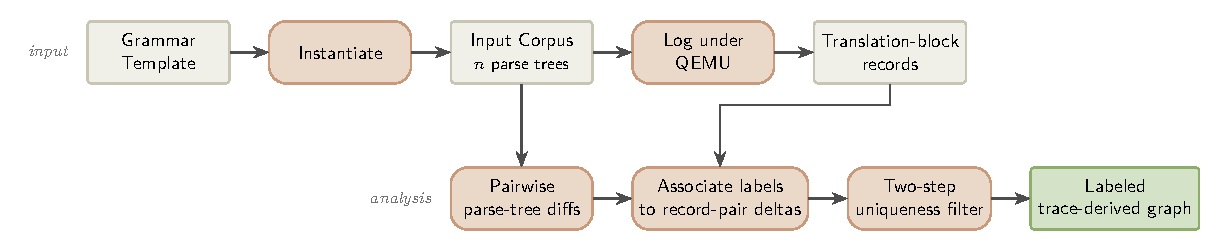
\includegraphics[width=0.92\linewidth]{figures/pipeline.pdf}
\caption{The \toolname pipeline. Cream rectangles are data artifacts. Salmon rounded rectangles are processing steps. The green rectangle is the final output. Vertical arrows bridge the two rows: the input corpus drives translation logging and pairwise input differencing, while the resulting block records feed label association.}
\label{fig:overview}
\end{figure*}

\subsection{Corpus Generation}\label{sec:design:corpus}

A grammar template is a tree of production rules.
Each leaf carries a small set of byte-level alternatives; each internal node carries a set of child configurations.
\toolname enumerates every combination of alternatives through Cartesian product, producing a corpus of concrete inputs each paired with its parse tree.

The templates are deliberately small.
The JSON template covers objects, arrays, strings, numbers, booleans, null, and a handful of degenerate cases (nan, inf), instantiating to 27 inputs.
The URI template covers scheme, authority, path, query, and fragment, instantiating to 1{,}458 inputs.
The ELF template, described in Section~\ref{sec:eval:elf}, instantiates to 20 inputs.

\textbf{The key property.}
For every pair of inputs we generate, the parse trees differ in either a single production or a small set of productions.
This is what makes attribution possible.
If two inputs differed in arbitrary ways, the trace differences between them could not be cleanly attributed to any single grammar element.

\subsection{Execution Tracing}\label{sec:design:trace}

Each input is fed to the target binary, which runs under \QEMU in user-mode emulation.
\QEMU logs translation blocks to a per-input file with each block's start address and disassembly.
\toolname parses the records into an ordered sequence, retains only blocks within the target binary's executable segment, and converts consecutive records into a trace-derived edge map.
These record pairs are useful differential signals, but the \texttt{-d in\_asm} translation log does not guarantee that every pair is a dynamic CFG edge.

Logs from inputs that the harness rejects (non-zero exit status) are dropped so the graph reflects only accepted corpus members.

\subsection{Label Association}\label{sec:design:assoc}

For every pair of inputs $(T_i, T_j)$ whose parse trees differ in exactly one production $p$, \toolname computes the consecutive-record-pair delta $E_i \setminus E_j$ and associates those pairs with $p$.
Aggregating over every input pair that isolates $p$ yields a per-production evidence set.

\textbf{Two-step uniqueness filter.}
Raw edge-to-label associations are noisy.
Many edges are shared across productions, including error-handling code and shared token-tape advancement.
\toolname strips this noise in two steps:

\begin{enumerate}
    \item \textbf{Subset removal.} If the edge set for production $p_1$ is nearly a subset of the edge set for $p_2$ ($|p_1 \setminus p_2| / |p_1| < 0.1$), \toolname removes $p_1$'s edges from $p_2$'s set. This eliminates setup and teardown code that runs for multiple productions but is most strongly associated with one.
    \item \textbf{Strict uniqueness.} For every production, \toolname subtracts the edges attributed to every other production. Edges that survive belong to a single production and receive its label.
\end{enumerate}

After filtering, \toolname propagates colors backward through the trace-derived graph.
A node whose outgoing edges all carry the same label is itself labeled with that color, which captures basic blocks that serve as sole entry points into a production-specific subgraph.

\subsection{Output}\label{sec:design:output}

\toolname emits three artifacts: a Graphviz DOT file of the labeled trace-derived graph, a rendered SVG for browser inspection, and an address-to-label mapping.
The mapping can be adapted for import into a disassembler, but this artifact does not yet include a dedicated import script.
